\documentclass[a4paper,10pt]{article}
\usepackage[utf8]{inputenc}
\usepackage[T1]{fontenc}
\usepackage[provide=*,french]{babel}
\usepackage[left=0.62cm,right=0.62cm,top=0.42cm,bottom=1.10cm]{geometry}
\usepackage{tikz}
\usepackage{graphicx}
\usepackage{xcolor}
\usepackage{eso-pic}
\usepackage{amssymb}
\usetikzlibrary{calc,patterns,arrows.meta}
\pagestyle{empty}
\renewcommand{\familydefault}{\sfdefault}
\setlength{\parindent}{0pt}

% Couleurs Maths&go / PythaBarre
\definecolor{brandNavy}{RGB}{11,53,112}
\definecolor{brandBlue}{RGB}{17,70,140}
\definecolor{brandTeal}{RGB}{29,174,174}
\definecolor{brandOrange}{RGB}{255,145,20}
\definecolor{softBlue}{RGB}{225,238,255}
\definecolor{softTeal}{RGB}{219,247,246}
\definecolor{softOrange}{RGB}{255,238,215}
\definecolor{softGreen}{RGB}{224,246,229}
\definecolor{softGray}{RGB}{245,247,250}
\definecolor{lightLine}{RGB}{190,230,230}

\newcommand{\LogoFile}{../assets/img/mathsgo-logo.png}
\newcommand{\MathsGoFooter}{%
\begin{tikzpicture}[remember picture,overlay]
  \node[anchor=south west,inner sep=0pt] at ([xshift=0.48cm,yshift=0.44cm]current page.south west)
    {\IfFileExists{\LogoFile}{\includegraphics[width=3.40cm]{\LogoFile}}{\tikz[baseline=-0.6ex]{\node[brandNavy,font=\sffamily\bfseries\fontsize{17}{18}\selectfont]{M};}}};
\end{tikzpicture}%
}
\AddToShipoutPictureFG{\MathsGoFooter}

% ---------- outils graphiques ----------
\newcommand{\LowDotted}[1]{%
\begin{tikzpicture}[baseline=-0.78ex]
  \draw[densely dotted, line width=0.95pt, line cap=round] (0,-0.22) -- (#1,-0.22);
\end{tikzpicture}}

% Pointillés placés plus bas sous une racine : laisse de l'air entre le trait de la racine et l'écriture de l'élève.
\newcommand{\RootBlank}[1]{\sqrt{\rule{0pt}{2.85ex}\;\smash{\raisebox{-0.92ex}{\LowDotted{#1}}}\;}}

\newcommand{\StepBadge}[1]{\tikz[baseline=-0.62ex]{\node[circle,fill=brandNavy,text=white,font=\bfseries,minimum size=0.60cm,inner sep=0pt]{#1};}}
\newcommand{\StepHead}[2]{\StepBadge{#1}\hspace{0.20cm}{\bfseries\color{brandNavy}\fontsize{13.6}{14.4}\selectfont #2}}
\newcommand{\SubHead}[2]{\textcolor{#1}{\bfseries\fontsize{12.1}{13.0}\selectfont #2}}
\newcommand{\CheckBox}{\ensuremath{\Box}\,}
\newcommand{\Sep}{\vspace{0.16cm}\noindent\textcolor{lightLine}{\rule{19.3cm}{0.42pt}}\vspace{0.14cm}}

% Moulin : mode 0 = vide, 1 = relation lettres, 2 = exemple hypotenuse, 3 = exemple cote.
\newcommand{\MoulinScale}[2]{%
\begin{tikzpicture}[scale=#2, line join=miter, line cap=round]
  \coordinate (A) at (0,0); \coordinate (B) at (0,1.22); \coordinate (C) at (1.63,0);
  \filldraw[fill=softBlue,draw=brandNavy,line width=0.85pt] (-1.22,0) rectangle (0,1.22);
  \filldraw[fill=softOrange,draw=brandNavy,line width=0.85pt] (0,-1.63) rectangle (1.63,0);
  \filldraw[fill=softGreen,draw=brandNavy,line width=0.85pt] (0,1.22) -- (1.63,0) -- (2.85,1.63) -- (1.22,2.85) -- cycle;
  \filldraw[fill=white,draw=brandNavy,line width=1.15pt] (A) -- (B) -- (C) -- cycle;
  \draw[brandNavy,line width=0.75pt] (0,0.18) -- (0.18,0.18) -- (0.18,0);
  \ifnum#1>0
    \node[brandNavy,font=\bfseries\large] at (-0.61,0.61) {$AB^2$};
    \node[brandNavy,font=\bfseries\large] at (0.82,-0.82) {$AC^2$};
    \node[brandNavy,font=\bfseries\large] at (1.48,1.54) {$BC^2$};
    \node[brandNavy,font=\bfseries\small] at (-0.17,-0.15) {$A$};
    \node[brandNavy,font=\bfseries\small] at (-0.17,1.37) {$B$};
    \node[brandNavy,font=\bfseries\small] at (1.81,-0.13) {$C$};
  \fi
  \ifnum#1=2
    \node[brandNavy,font=\bfseries\small] at (0.30,0.66) {$3$};
    \node[brandNavy,font=\bfseries\small] at (0.82,-0.16) {$4$};
    \node[brandNavy,font=\bfseries\large] at (0.75,0.50) {?};
  \fi
  \ifnum#1=3
    \node[brandNavy,font=\bfseries\small] at (0.78,0.76) {$5$};
    \node[brandNavy,font=\bfseries\small] at (0.82,-0.16) {$4$};
    \node[brandNavy,font=\bfseries\large] at (0.28,0.55) {?};
  \fi
\end{tikzpicture}}
\newcommand{\Moulin}[1]{\MoulinScale{#1}{1.70}}
\newcommand{\MoulinMini}[1]{\MoulinScale{#1}{0.76}}

% Tableaux PythaBarre
\newcommand{\BarTwo}[9]{%
\begin{tikzpicture}[x=1cm,y=1cm]
  \def\W{#9}\def\H{0.78}
  \pgfmathsetmacro{\Split}{\W*(#1)/(#1+#2)}
  \draw[rounded corners=1pt,fill=#6,draw=brandNavy!80,line width=0.85pt] (0,\H) rectangle (\W,{2*\H});
  \node[font=\bfseries\fontsize{12.9}{13.5}\selectfont\color{brandNavy}] at ({\W/2},{1.5*\H}) {#3};
  \draw[rounded corners=1pt,fill=#7,draw=brandNavy!80,line width=0.85pt] (0,0) rectangle (\Split,\H);
  \draw[rounded corners=1pt,fill=#8,draw=brandNavy!80,line width=0.85pt] (\Split,0) rectangle (\W,\H);
  \node[font=\bfseries\fontsize{12.9}{13.5}\selectfont\color{brandNavy}] at ({\Split/2},{0.5*\H}) {#4};
  \node[font=\bfseries\fontsize{12.9}{13.5}\selectfont\color{brandNavy}] at ({(\Split+\W)/2},{0.5*\H}) {#5};
\end{tikzpicture}}

\newcommand{\BarOne}[5]{%
\begin{tikzpicture}[x=1cm,y=1cm]
  \def\W{#5}\def\H{0.78}
  \draw[rounded corners=1pt,fill=#3,draw=brandNavy!80,line width=0.85pt] (0,\H) rectangle (\W,{2*\H});
  \node[font=\bfseries\fontsize{12.9}{13.5}\selectfont\color{brandNavy}] at ({\W/2},{1.5*\H}) {#1};
  \draw[rounded corners=1pt,fill=#4,draw=brandNavy!80,line width=0.85pt] (0,0) rectangle (\W,\H);
  \node[font=\bfseries\fontsize{12.9}{13.5}\selectfont\color{brandNavy}] at ({\W/2},{0.5*\H}) {#2};
\end{tikzpicture}}

% Encadrements colorés des termes de l'équation.
% Les bulles reprennent exactement les couleurs de remplissage des tableaux.
\newcommand{\TermColorBox}[3]{\tikz[baseline=-0.72ex]{\node[rounded corners=4pt,draw=#1,fill=#2,line width=0.78pt,inner xsep=5pt,inner ysep=4.5pt,minimum width=2.48cm,minimum height=0.72cm,font=\bfseries\fontsize{12.7}{13.4}\selectfont\color{brandNavy}]{#3};}}
\newcommand{\TermH}[1]{\TermColorBox{brandTeal}{softGreen}{#1}}
\newcommand{\TermB}[1]{\TermColorBox{brandBlue}{softBlue}{#1}}
\newcommand{\TermO}[1]{\TermColorBox{brandOrange}{softOrange}{#1}}
\newcommand{\TermBox}[2]{\TermColorBox{#1}{#1!10}{#2}}
\newcommand{\TermBoxN}[1]{\tikz[baseline=-0.72ex]{\node[rounded corners=4pt,draw=brandNavy!45,fill=softGray,line width=0.72pt,inner xsep=5pt,inner ysep=4.5pt,minimum width=2.48cm,minimum height=0.72cm,font=\bfseries\fontsize{12.7}{13.4}\selectfont\color{brandNavy}]{#1};}}
\newcommand{\EqColor}[3]{\TermH{#1}\;=\;\TermB{#2}\;+\;\TermO{#3}}
\newcommand{\EqNeutralSub}[3]{\TermBoxN{#1}\;-\;\TermBoxN{#2}\;=\;\TermBoxN{#3}}
\newcommand{\EqNeutral}[2]{\TermBoxN{#1}\;=\;\TermBoxN{#2}}
\newcommand{\AnswerBox}[2]{\tikz[baseline=-0.72ex]{\node[rounded corners=6pt,draw=#1,fill=white,line width=0.85pt,inner xsep=8pt,inner ysep=5.5pt,text width=#2,align=center,font=\bfseries\fontsize{12.1}{13.0}\selectfont\color{brandNavy}]{Donc \LowDotted{2.15} mesure \LowDotted{2.05}.};}}

\newcommand{\ToolRow}[2]{%
\noindent\begin{minipage}[c]{8.20cm}\centering #1\end{minipage}\hfill%
\begin{minipage}[c]{10.25cm}\centering #2\end{minipage}\par\vspace{0.23cm}}

\newcommand{\ConclusionBox}[2]{%
\begin{tikzpicture}
\node[rounded corners=6pt,draw=#1,fill=white,line width=0.85pt,inner sep=9.5pt,text width=#2,align=center,font=\bfseries\fontsize{12.1}{13.0}\selectfont\color{brandNavy}] \bgroup
}
\newcommand{\EndConclusion}{\egroup;\end{tikzpicture}}

\newcommand{\HeaderPythagore}{%
\noindent\begin{minipage}[c]{0.43\textwidth}
  \centering \Moulin{0}
\end{minipage}%
\hfill
\begin{minipage}[c]{0.55\textwidth}
  \begin{center}
  {\fontsize{30}{31}\selectfont\bfseries\color{brandNavy} Théorème de}\par\vspace{-0.01cm}
  {\fontsize{30}{31}\selectfont\bfseries\color{brandNavy} Pythagore}\par\vspace{0.12cm}
  {\fontsize{11.7}{12.8}\selectfont\bfseries\color{brandTeal} Objectif : calculer une longueur en utilisant le théorème de Pythagore.}\par\vspace{0.16cm}
  
\begin{tikzpicture}
  \node[rounded corners=7pt,draw=brandOrange!70,fill=softOrange!65,line width=0.75pt,text width=9.75cm,inner sep=7pt,align=center,font=\bfseries\fontsize{10.1}{11.2}\selectfont\color{brandNavy}] {Si un triangle est rectangle, alors le carré de l'\mbox{hypoténuse} est égal à la somme des carrés des deux autres côtés.};
  \end{tikzpicture}
  \end{center}
\end{minipage}\par\vspace{0.52cm}}

\newcommand{\PageNote}[1]{%
\vfill
\begin{center}
\begin{tikzpicture}
  \node[rounded corners=7pt, fill=softBlue!50, draw=brandNavy!25, line width=0.6pt, text width=17.4cm, inner sep=5pt, align=center]
  {\small\bfseries\color{brandNavy} #1};
\end{tikzpicture}
\end{center}\vspace{0.76cm}}


\begin{document}

% ================= PAGE 1 - Élève : outil de calcul =================
\HeaderPythagore

\StepHead{1}{Je complète ma figure}\par\vspace{0.17cm}
{\small\bfseries\color{brandNavy} Je nomme les sommets, j'indique les longueurs que je connais et celle que je cherche. Je repère l'hypoténuse et les deux côtés de l'angle droit.}\par\vspace{0.34cm}

\StepHead{2}{J'explique ce que je fais, puis j'écris l'égalité de Pythagore}\par\vspace{0.17cm}
{\fontsize{10.8}{11.7}\selectfont Le triangle \LowDotted{2.25} est rectangle en \LowDotted{1.05}, donc je peux appliquer le théorème de Pythagore. On a :}\par\vspace{0.23cm}
\ToolRow{\BarTwo{1}{1}{$\LowDotted{1.85}^{\;2}$}{$\LowDotted{1.85}^{\;2}$}{$\LowDotted{1.85}^{\;2}$}{softGreen}{softBlue}{softOrange}{7.65}}{\EqColor{$\LowDotted{1.70}^{\;2}$}{$\LowDotted{1.70}^{\;2}$}{$\LowDotted{1.70}^{\;2}$}}
{\bfseries\fontsize{11.3}{12}\selectfont\color{brandNavy} Je remplace les longueurs connues.}\par\vspace{0.13cm}
\ToolRow{\BarTwo{1}{1}{$\LowDotted{1.85}^{\;2}$}{$\LowDotted{1.85}^{\;2}$}{$\LowDotted{1.85}^{\;2}$}{softGreen}{softBlue}{softOrange}{7.65}}{\EqColor{$\LowDotted{1.70}^{\;2}$}{$\LowDotted{1.70}^{\;2}$}{$\LowDotted{1.70}^{\;2}$}}
{\bfseries\fontsize{11.3}{12}\selectfont\color{brandNavy} Je calcule les carrés connus.}\par\vspace{0.13cm}
\ToolRow{\BarTwo{1}{1}{$\LowDotted{1.85}$}{$\LowDotted{1.85}$}{$\LowDotted{1.85}$}{softGreen}{softBlue}{softOrange}{7.65}}{\EqColor{$\LowDotted{1.70}$}{$\LowDotted{1.70}$}{$\LowDotted{1.70}$}}
\Sep

\StepHead{3}{Je choisis le bon chemin}\par\vspace{0.19cm}
\noindent\begin{minipage}[t]{9.35cm}
\vspace{0pt}
{\SubHead{brandTeal}{\CheckBox Chemin A : je cherche l'hypoténuse}}\par\vspace{0.08cm}

\begin{tikzpicture}
\node[rounded corners=7pt,draw=brandTeal,fill=brandTeal!5,line width=0.85pt,text width=8.95cm,inner sep=8pt] {\centering
\begin{tabular}{r@{\;}c@{\;}l}
\TermH{$\LowDotted{1.70}^{\;2}$} & = & \TermH{$\LowDotted{1.95}$}
\end{tabular}\par\vspace{0.20cm}
{\fontsize{9.6}{10.5}\selectfont\bfseries\color{brandTeal} Je regroupe les deux carrés connus.}\par\vspace{0.05cm}
};
\end{tikzpicture}
\end{minipage}\hfill
\begin{minipage}[t]{9.35cm}
\vspace{0pt}
{\SubHead{brandOrange}{\CheckBox Chemin B : je cherche un côté de l'angle droit}}\par\vspace{0.08cm}
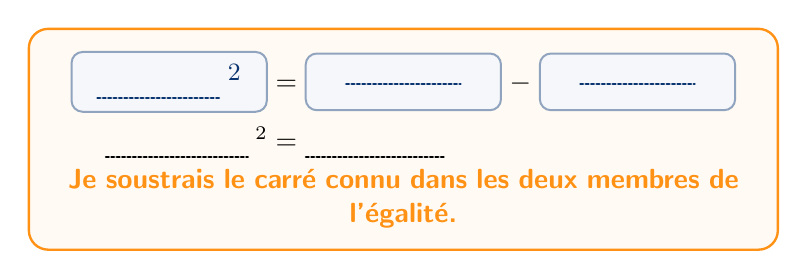
\begin{tikzpicture}
\node[rounded corners=7pt,draw=brandOrange,fill=brandOrange!5,line width=0.85pt,text width=8.95cm,inner sep=8pt] {\centering
\begin{tabular}{r@{\;}c@{\;}l}
\TermBoxN{$\LowDotted{1.55}^{\;2}$} & = & \TermBoxN{$\LowDotted{1.45}$}\;$-$\;\TermBoxN{$\LowDotted{1.45}$}\\[0.32cm]
$\LowDotted{1.80}^{\;2}$ & = & $\LowDotted{1.75}$
\end{tabular}\par\vspace{0.10cm}
{\fontsize{9.6}{10.5}\selectfont\bfseries\color{brandOrange} Je soustrais le carré connu dans les deux membres de l'égalité.}\par\vspace{0.03cm}
};
\end{tikzpicture}
\end{minipage}

\vspace{0.12cm}
\StepHead{4}{Je passe du carré à la longueur}\par\vspace{0.06cm}
\begin{center}
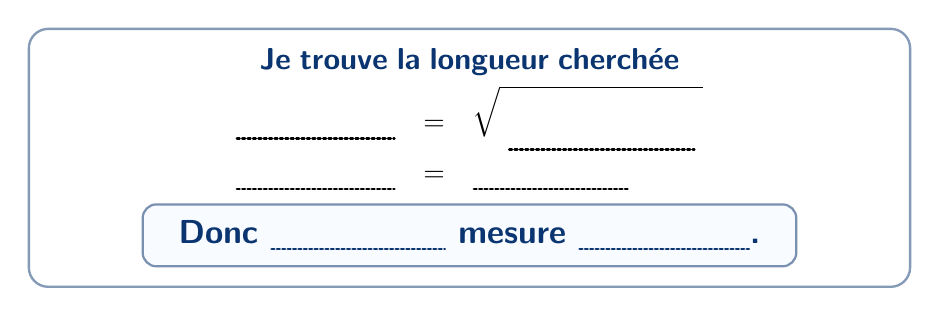
\begin{tikzpicture}[>=Latex]
  \draw[brandTeal,line width=0.85pt,->] (-4.25,0.12) -- (-1.78,-0.55);
  \draw[brandOrange,line width=0.85pt,->] (4.25,0.12) -- (1.78,-0.55);
  \node[rounded corners=7pt,draw=brandNavy!50,fill=white,line width=0.85pt,text width=10.7cm,inner sep=7.0pt,align=center] at (0,-1.27) {%
  {\bfseries\fontsize{11.4}{12.2}\selectfont\color{brandNavy} Je trouve la longueur cherchée}\par\vspace{0.10cm}
  $\begin{array}{rcl}
  \LowDotted{2.00} & = & \RootBlank{2.35}\\[0.22cm]
  \LowDotted{2.00} & = & \LowDotted{1.95}
  \end{array}$\par\vspace{0.12cm}
  \tikz[baseline=-0.72ex]{\node[rounded corners=5pt,draw=brandNavy!55,fill=softBlue!25,line width=0.8pt,inner xsep=13pt,inner ysep=5.8pt,font=\bfseries\fontsize{12.1}{13.0}\selectfont\color{brandNavy}]{Donc \LowDotted{2.20} mesure \LowDotted{2.15}.};}
  };
\end{tikzpicture}
\end{center}

\vspace{-0.15cm}
\begin{center}

\begin{tikzpicture}
  \node[rounded corners=7pt,fill=softOrange!55,draw=brandOrange!55,line width=0.6pt,text width=16.9cm,inner sep=5pt,align=center] {\small\bfseries\color{brandNavy} Je vérifie : l'hypoténuse est-elle bien plus grande que les deux autres côtés ? \hspace{0.35cm} $\Box$ oui \hspace{0.30cm} $\Box$ non};
\end{tikzpicture}
\end{center}

\newpage





% ================= PAGE 2 - Élève : rédaction propre avec repères à gauche =================
\begin{center}
{\fontsize{27}{29}\selectfont\bfseries\color{brandNavy} Théorème de Pythagore}\par\vspace{0.04cm}
{\fontsize{15}{16}\selectfont\bfseries\color{brandTeal} Rédaction propre pour la résolution de problème}
\end{center}\vspace{0.18cm}


\noindent
\begin{minipage}[t]{5.70cm}
\vspace{0pt}
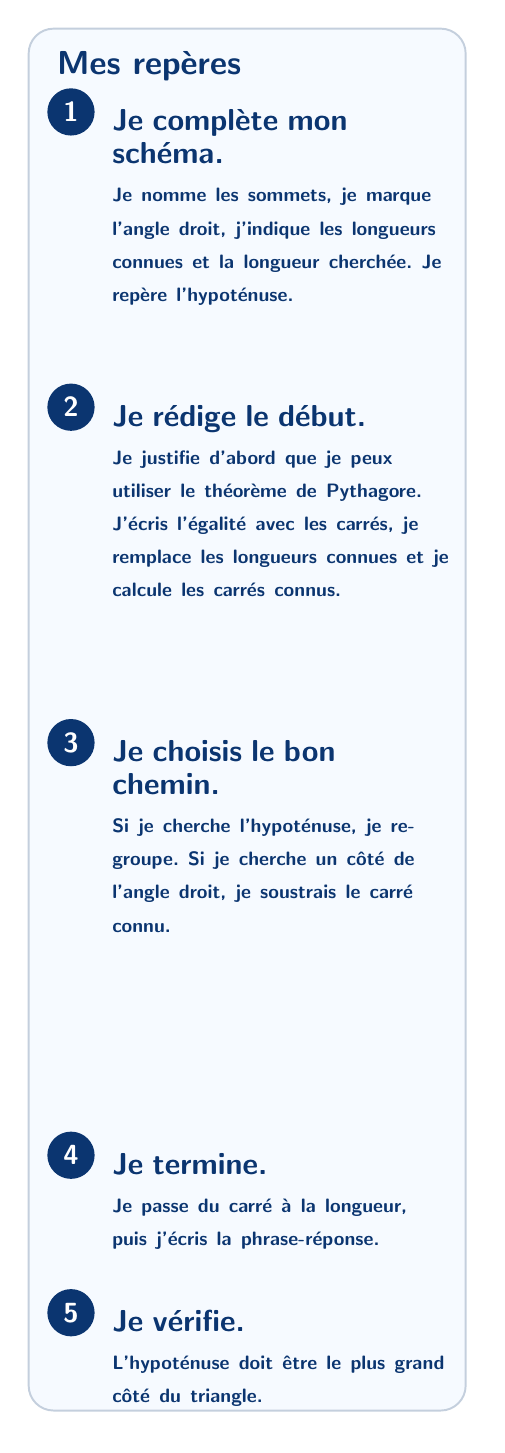
\begin{tikzpicture}[x=1cm,y=1cm]
\path[use as bounding box] (0,0) rectangle (5.70,-17.75);
\node[rounded corners=9pt,draw=brandNavy!24,fill=softBlue!30,line width=0.70pt,minimum width=5.55cm,minimum height=17.55cm,anchor=north west] at (0,0) {};
\node[anchor=north west,text=brandNavy,font=\bfseries\fontsize{12.6}{13.6}\selectfont] at (0.25,-0.18) {Mes repères};

% Repère 1 - aligné avec le schéma
\node[circle,fill=brandNavy,text=white,font=\bfseries,minimum size=0.60cm,inner sep=0pt] at (0.55,-1.07) {1};
\node[anchor=north west,text width=4.30cm,align=left] at (0.95,-0.92) {\bfseries\color{brandNavy}\fontsize{11.1}{11.9}\selectfont Je complète mon schéma.\par\vspace{0.06cm}
{\scriptsize\bfseries\color{brandNavy} Je nomme les sommets, je marque l'angle droit, j'indique les longueurs connues et la longueur cherchée. Je repère l'hypoténuse.}};

% Repère 2 - aligné avec le cadre de rédaction du début
\node[circle,fill=brandNavy,text=white,font=\bfseries,minimum size=0.60cm,inner sep=0pt] at (0.55,-4.82) {2};
\node[anchor=north west,text width=4.30cm,align=left] at (0.95,-4.67) {\bfseries\color{brandNavy}\fontsize{11.1}{11.9}\selectfont Je rédige le début.\par\vspace{0.06cm}
{\scriptsize\bfseries\color{brandNavy} Je justifie d'abord que je peux utiliser le théorème de Pythagore. J'écris l'égalité avec les carrés, je remplace les longueurs connues et je calcule les carrés connus.}};

% Repère 3 - aligné avec le choix du chemin
\node[circle,fill=brandNavy,text=white,font=\bfseries,minimum size=0.60cm,inner sep=0pt] at (0.55,-9.08) {3};
\node[anchor=north west,text width=4.30cm,align=left] at (0.95,-8.93) {\bfseries\color{brandNavy}\fontsize{11.1}{11.9}\selectfont Je choisis le bon chemin.\par\vspace{0.06cm}
{\scriptsize\bfseries\color{brandNavy} Si je cherche l'hypoténuse, je regroupe. Si je cherche un côté de l'angle droit, je soustrais le carré connu.}};

% Repère 4 - aligné avec la phrase-réponse
\node[circle,fill=brandNavy,text=white,font=\bfseries,minimum size=0.60cm,inner sep=0pt] at (0.55,-14.32) {4};
\node[anchor=north west,text width=4.30cm,align=left] at (0.95,-14.17) {\bfseries\color{brandNavy}\fontsize{11.1}{11.9}\selectfont Je termine.\par\vspace{0.06cm}
{\scriptsize\bfseries\color{brandNavy} Je passe du carré à la longueur, puis j'écris la phrase-réponse.}};

% Repère 5 - aligné avec la vérification
\node[circle,fill=brandNavy,text=white,font=\bfseries,minimum size=0.60cm,inner sep=0pt] at (0.55,-16.32) {5};
\node[anchor=north west,text width=4.30cm,align=left] at (0.95,-16.17) {\bfseries\color{brandNavy}\fontsize{11.1}{11.9}\selectfont Je vérifie.\par\vspace{0.06cm}
{\scriptsize\bfseries\color{brandNavy} L'hypoténuse doit être le plus grand côté du triangle.}};
\end{tikzpicture}
\end{minipage}\hfill
\begin{minipage}[t]{13.05cm}
\vspace{0pt}
% --- 1 : schéma ---
{\bfseries\color{brandTeal}\fontsize{10.8}{11.4}\selectfont Je peux surligner l'hypoténuse sur mon schéma.}\par\vspace{0.06cm}
\begin{center}
\begin{tikzpicture}
\node[rounded corners=8pt,draw=brandTeal!65,fill=brandTeal!3,line width=0.75pt,text width=12.25cm,inner sep=7pt,align=center] {
\begin{tikzpicture}[x=1cm,y=1cm,line cap=butt,line join=miter]
  \coordinate (A) at (0,0); \coordinate (B) at (0,1.75); \coordinate (C) at (4.25,0);
  \fill[white] (A) -- (B) -- (C) -- cycle;
  % Vrai triangle rectangle : côté vertical, côté horizontal, hypoténuse droite.
  \draw[brandNavy,line width=1.25pt] (A) -- (B);
  \draw[brandNavy,line width=1.25pt] (A) -- (C);
  \draw[brandTeal,line width=4.4pt,opacity=.24] (B) -- (C);
  \draw[brandNavy,line width=1.25pt] (B) -- (C);
  % Codage de l'angle droit : uniquement les deux traits intérieurs du petit carré.
  % Les deux côtés extérieurs sont déjà portés par les côtés du triangle.
  \draw[brandNavy,line width=1.05pt,sharp corners,line cap=butt,line join=miter] (0,0.34) -- (0.34,0.34) -- (0.34,0);
  \node[brandNavy!70,font=\bfseries\small] at (-0.37,-0.22) {\LowDotted{0.70}};
  \node[brandNavy!70,font=\bfseries\small] at (-0.37,1.97) {\LowDotted{0.70}};
  \node[brandNavy!70,font=\bfseries\small] at (4.58,-0.22) {\LowDotted{0.70}};
  \node[brandNavy!70,font=\bfseries\small] at (-0.55,0.88) {\LowDotted{0.86}};
  \node[brandNavy!70,font=\bfseries\small] at (2.12,-0.28) {\LowDotted{0.86}};
  \node[brandNavy!70,font=\bfseries\small] at (2.22,1.06) {\LowDotted{0.86}};
\end{tikzpicture}
};
\end{tikzpicture}
\end{center}

\vspace{0.10cm}
% --- 2 : rédaction commune ---
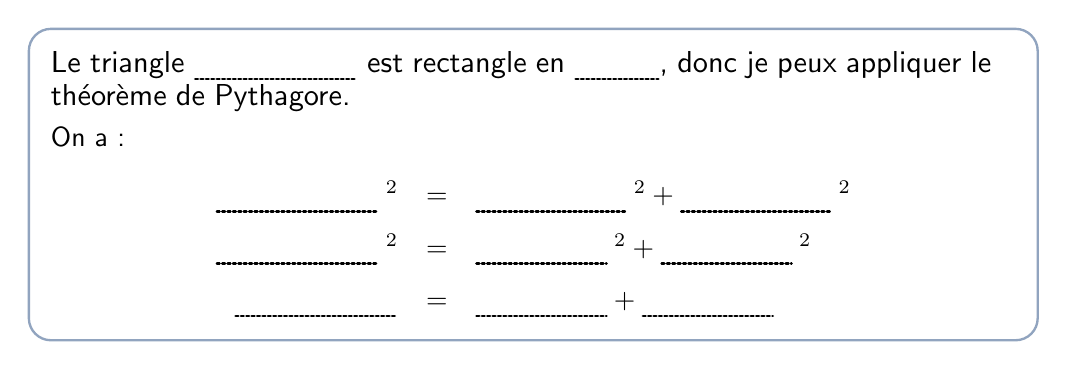
\begin{tikzpicture}
\node[rounded corners=8pt,draw=brandNavy!45,fill=white,line width=0.85pt,text width=12.25cm,inner sep=8pt,align=left] {
{\fontsize{10.5}{12.4}\selectfont
Le triangle \LowDotted{2.05} est rectangle en \LowDotted{1.05}, donc je peux appliquer le théorème de Pythagore.}\par\vspace{0.10cm}
On a :\par\vspace{0.05cm}
\begin{center}
$\begin{array}{rcl}
\LowDotted{2.05}^{\;2} & = & \LowDotted{1.90}^{\;2} + \LowDotted{1.90}^{\;2}\\[0.24cm]
\LowDotted{2.05}^{\;2} & = & \LowDotted{1.65}^{\;2} + \LowDotted{1.65}^{\;2}\\[0.24cm]
\LowDotted{2.05}       & = & \LowDotted{1.65} + \LowDotted{1.65}
\end{array}$
\end{center}
};
\end{tikzpicture}

\vspace{0.18cm}
% --- 3 : choix du chemin ---
\noindent\begin{minipage}[t]{6.18cm}
\vspace{0pt}
{\bfseries\color{brandTeal}\fontsize{11.6}{12.3}\selectfont \CheckBox Chemin A : je cherche l'hypoténuse}\par\vspace{0.06cm}
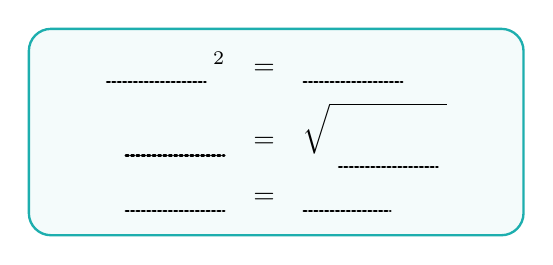
\begin{tikzpicture}
\node[rounded corners=8pt,draw=brandTeal,fill=brandTeal!5,line width=0.85pt,text width=5.72cm,inner sep=8pt,align=center] {
$\begin{array}{rcl}
\LowDotted{1.25}^{\;2} & = & \LowDotted{1.25}\\[0.24cm]
\LowDotted{1.25}       & = & \RootBlank{1.25}\\[0.28cm]
\LowDotted{1.25}       & = & \LowDotted{1.10}
\end{array}$
};
\end{tikzpicture}
\end{minipage}\hfill
\begin{minipage}[t]{6.18cm}
\vspace{0pt}
{\bfseries\color{brandOrange}\fontsize{11.6}{12.3}\selectfont \CheckBox Chemin B : je cherche un côté de l'angle droit}\par\vspace{0.06cm}
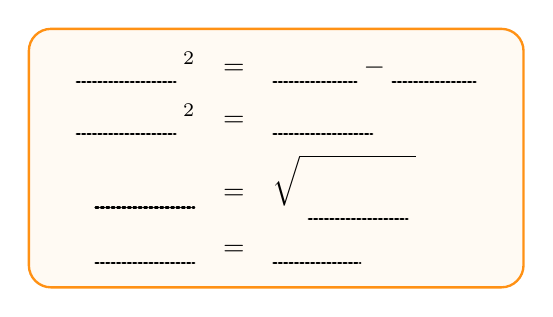
\begin{tikzpicture}
\node[rounded corners=8pt,draw=brandOrange,fill=brandOrange!5,line width=0.85pt,text width=5.72cm,inner sep=8pt,align=center] {
$\begin{array}{rcl}
\LowDotted{1.25}^{\;2} & = & \LowDotted{1.05} - \LowDotted{1.05}\\[0.24cm]
\LowDotted{1.25}^{\;2} & = & \LowDotted{1.25}\\[0.24cm]
\LowDotted{1.25}       & = & \RootBlank{1.25}\\[0.28cm]
\LowDotted{1.25}       & = & \LowDotted{1.10}
\end{array}$
};
\end{tikzpicture}
\end{minipage}

\vspace{0.58cm}
% --- 4 : conclusion commune ---
\begin{center}
\tikz[baseline=-0.72ex]{\node[rounded corners=6pt,draw=brandNavy!55,fill=softBlue!18,line width=0.8pt,inner xsep=24pt,inner ysep=7pt,font=\bfseries\fontsize{12.5}{13.3}\selectfont\color{brandNavy}]{Donc \LowDotted{2.65} mesure \LowDotted{2.55}.};}
\end{center}

\vspace{0.08cm}
% --- 5 : vérification ---
\begin{center}
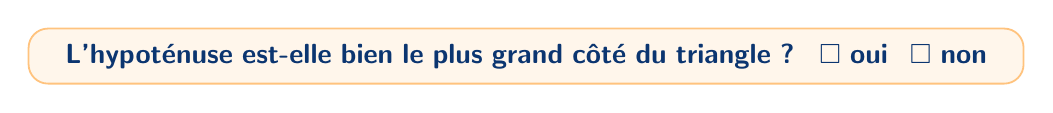
\begin{tikzpicture}
\node[rounded corners=7pt,draw=brandOrange!55,fill=softOrange!50,line width=0.65pt,text width=12.25cm,inner sep=5.5pt,align=center] {\bfseries\color{brandNavy} L'hypoténuse est-elle bien le plus grand côté du triangle ? \hspace{0.20cm}$\Box$ oui \hspace{0.16cm}$\Box$ non};
\end{tikzpicture}
\end{center}
\end{minipage}

\end{document}
